\documentclass{article}

\usepackage{array}
\usepackage{graphicx}

\begin{document}

\title{Faraday's Law, Problems}
\author{GSI: Caleb Eades}
\date{11/20}
\maketitle

\section{Faraday's Law}

\subsection{Alternating Current through Rotations}

Alternating current generator. A rectangular loop of $N$ turns with length $a$ and width $b$ is rotated at an angular frequency $\omega$ in a uniform field of induction $\vec{B}$. Show that there is an induced EMF $\epsilon = \omega Nba B \sin \omega t = \epsilon_0 \sin \omega t$.

\textit{(Source: Halliday and Resnick, Problem 35.9)}

\subsection{Falling Rails}

A rod with length $l$, mass $m$, and resistance $R$ slides without friction down parallel conducting rails of negligible resistance, as shown below. The plane of the rails makes an angle $\theta$ with the horizontal, and a uniform vertical magnetic field $\vec{B}$ exists throughout the region.
\begin{itemize}
	\item[(a)] Find the steady-state terminal velocity of the sliding rod.
	\item[(b)] Show that the rate at which the internal energy of the rod is increasing is equal to the rate at which the rod is losing gravitational potential energy.
	\item[(c)] Discuss the situation if $\vec{B}$ were directed down instead of up.
\end{itemize}

\textit{(Source: Halliday, Resnick, Krane 34.9)}

\section{Previous Exam Problems}

A long straight wire of radius $\rho$ carries a current along its axis with a non-uniform current density $j(r)=mr^2$ ($m$=constant), $r$ being the radial distance measured from the symmetry axis of the wire, as shown below.
\begin{itemize}
	\item[(a)] Calculate the magnitude of the magnetic field produced inside and outside the wire.
	\item[(b)] Draw some field lines to show qualitatively how the magnitude and direction of the magnetic field vary. Specify the direction of the current in your drawing.
	\item[(c)] A rectangular loop of sides $a$ and $b$ and resistance $R$ is placed a distance $d$ ($d>\rho$) from the center of the current-carrying wire, as shown below. What is the induced current in the lop if it is (i) translated along the $y$-axis at constant speed $v$? (ii) translated along the $x$-axis at speed $v$?
\end{itemize}
\begin{figure}[h]
\begin{center}
	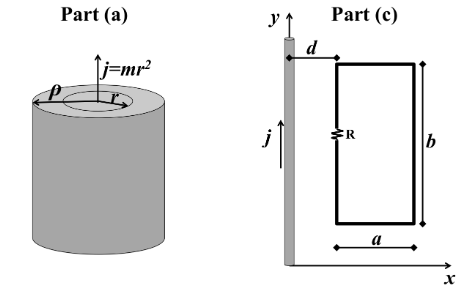
\includegraphics[width=0.5\textwidth]{cylinderinduced.png}
\end{center}
\end{figure}

\textit{(Source: Birgeneau, Fall 2015 Final Exam, Problem 4)}

\subsection{Loops and Forces}

The figure shows a wire loop, which has a length, $l$, and width, $w$, inside a magnetic field, $B$. The loop is made of a wire with resistivity, $\rho$, and cross-sectional area, $A$. A crossbar made of a conducting metal with negligible resistance is in contact with the loop, and at the instant shown in the figure, it has velocity, $v$, and there are currents on both sides of the bar. What force, $F$, (magnitude and direction) must be placed on the rod when it is at the position shown so that the velocity of the rod is constant?
\begin{figure}[h]
	\begin{center}
		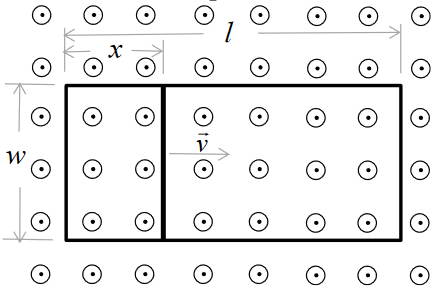
\includegraphics[width=0.5\textwidth]{wireloops.png}
	\end{center}
\end{figure}

\textit{(Source: Speliotopoulos, Fall 2012 Final Exam, Problem 3)}

\end{document}
